\section{Results}

\subsection{Target Trial Emulation}

\begin{figure}
    \centering
    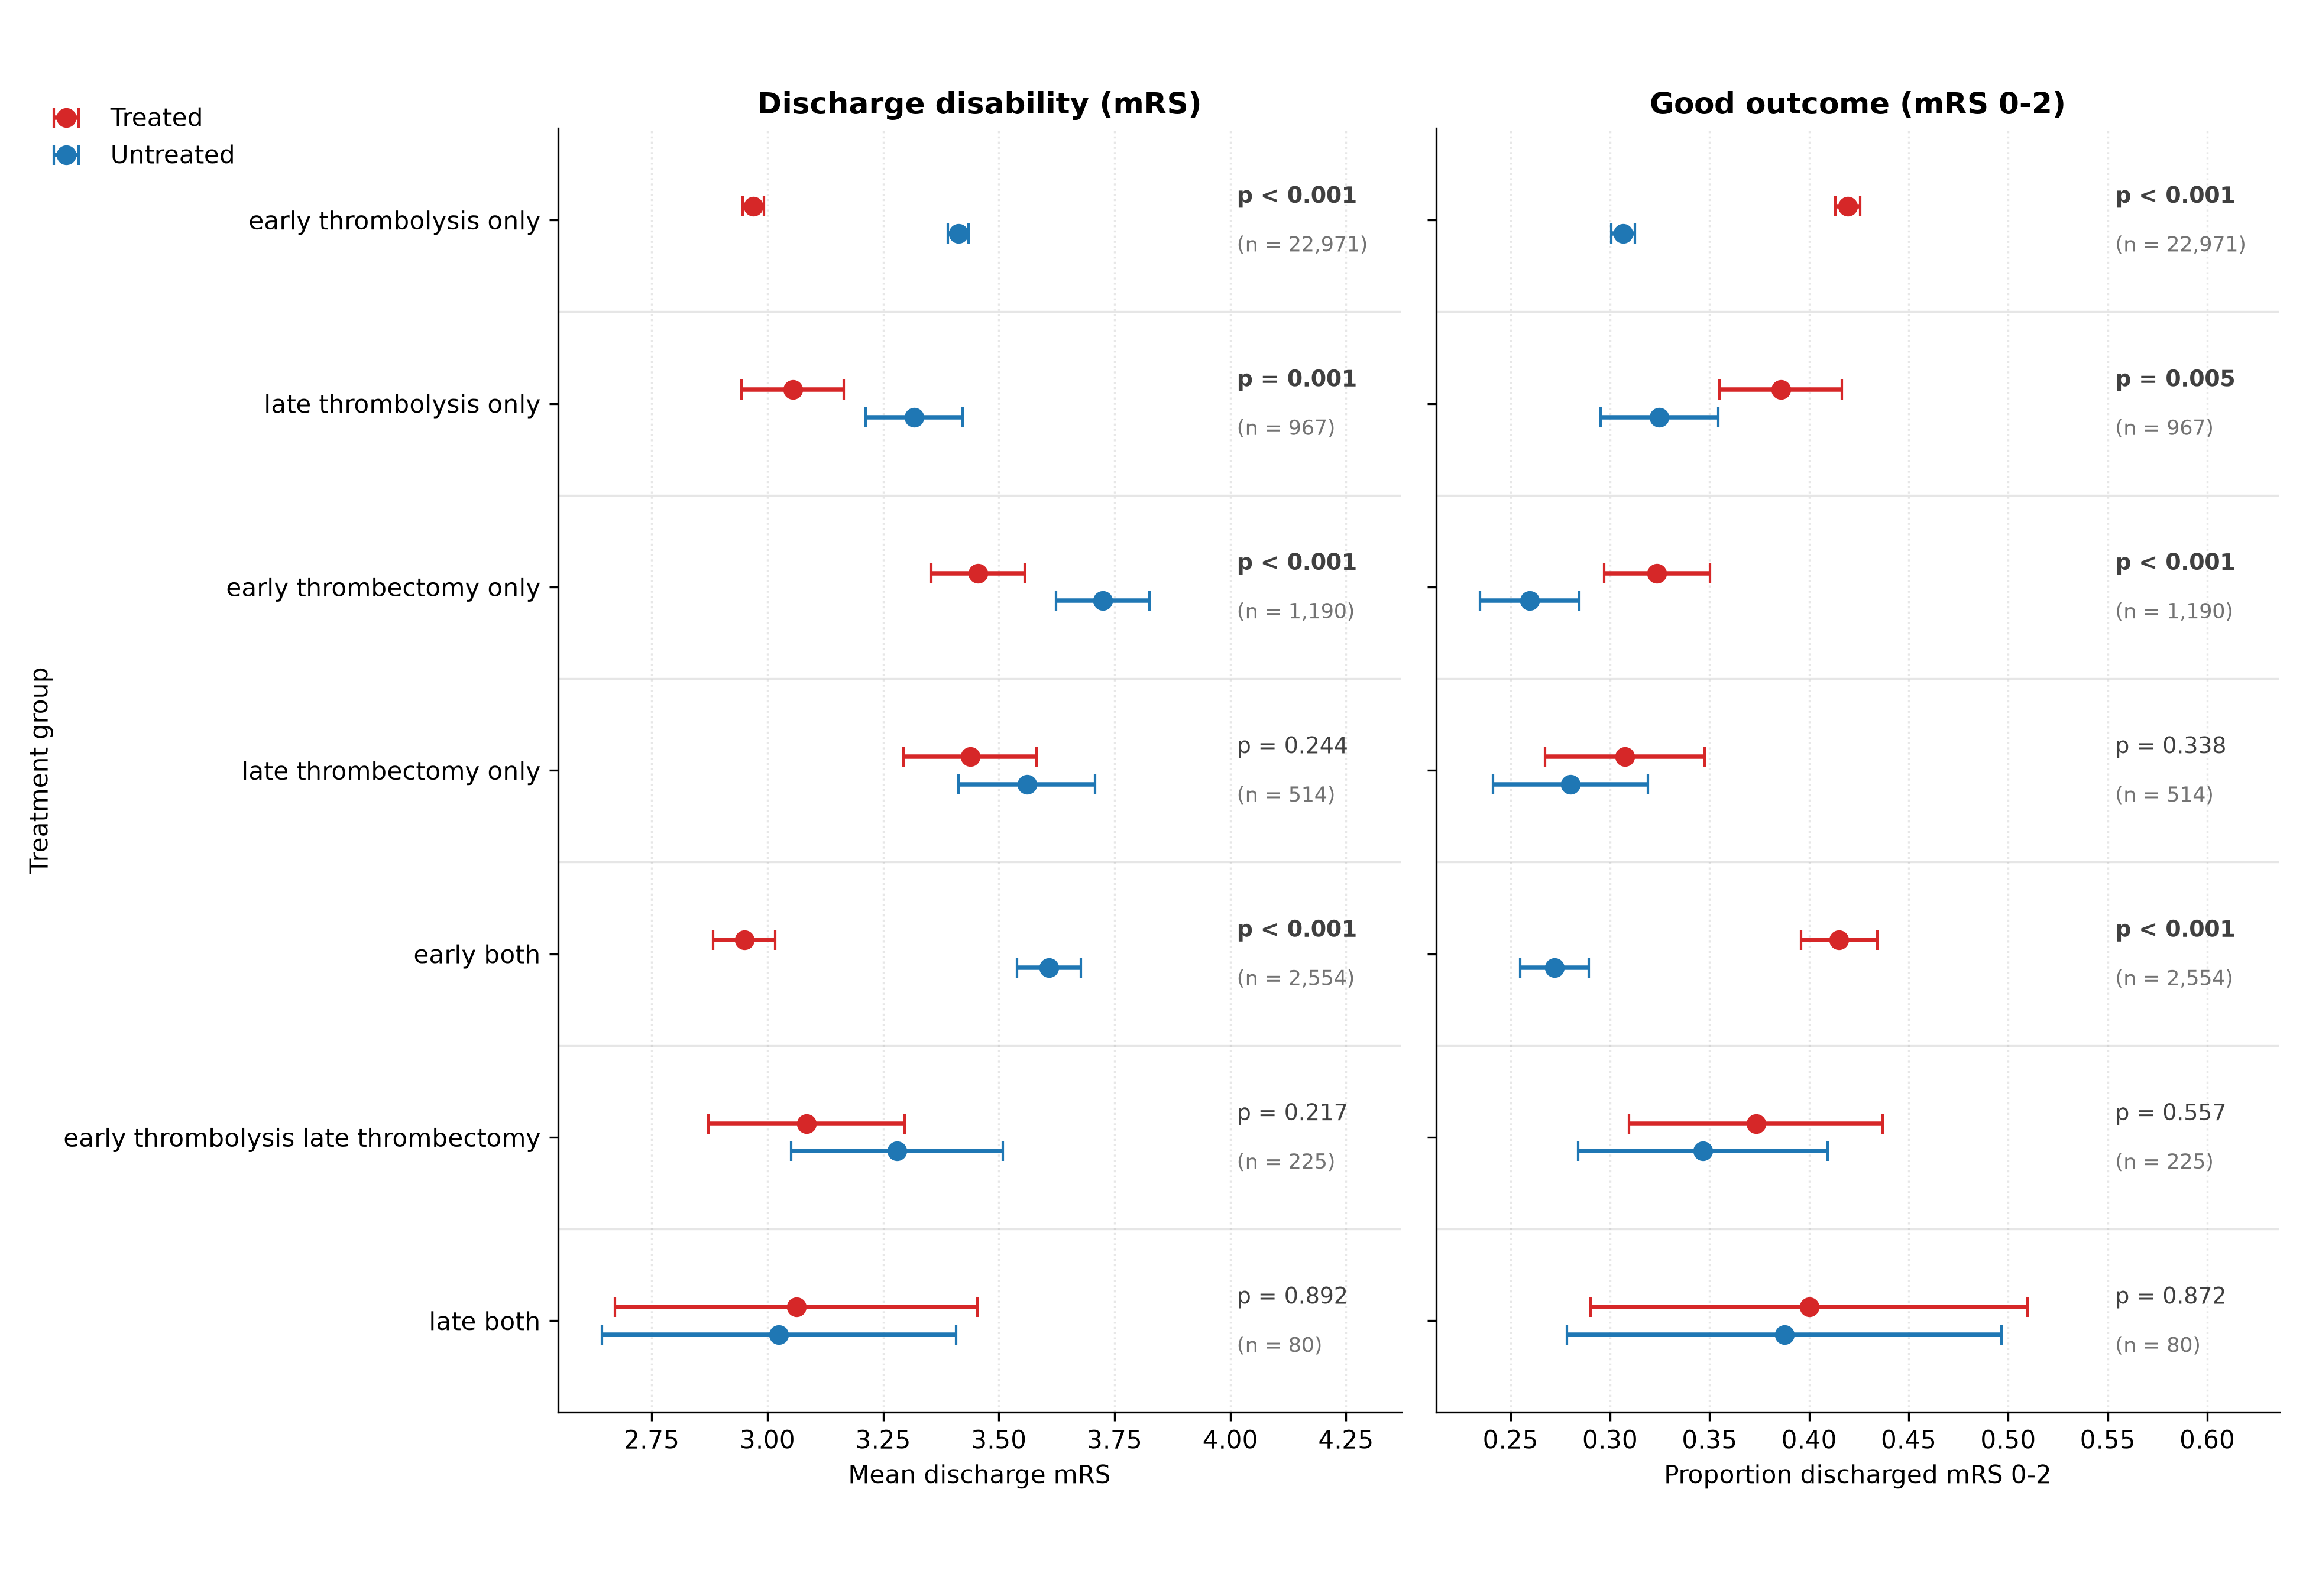
\includegraphics[width=1\linewidth]{images/treatment_effects/target_trial_emulation_mrs_2.png}
    \caption{Target trial emulation of reperfusion-treatment timing strategies and discharge functional outcomes, using matched control and treated patients. Estimated mean discharge modified Rankin Scale (mRS; left panel) and proportion achieving an outcome of mRS 0–2 (right panel) are shown for patients receiving each treatment strategy (red) and their emulated untreated comparators (blue). Strategies are defined by early ($<$ 270 mins from onset) or late ($\geq$ 270 mins from onset) intravenous thrombolysis, mechanical thrombectomy, or their combination. Points denote estimated outcomes and horizontal bars 95\% confidence intervals; p-values indicate the treated–untreated comparison within each emulated treatment group, with sample sizes shown. Lower mRS and higher mRS 0–2 proportions indicate more favourable outcomes.}
    \label{fig:main_target_trial_mrs_2}
\end{figure}

\subsection{S-Learner}

%% SHAP All patients

\begin{figure}[htbp]
    \centering
    
    % Top image (Full width)
    \begin{subfigure}{0.50\textwidth}
        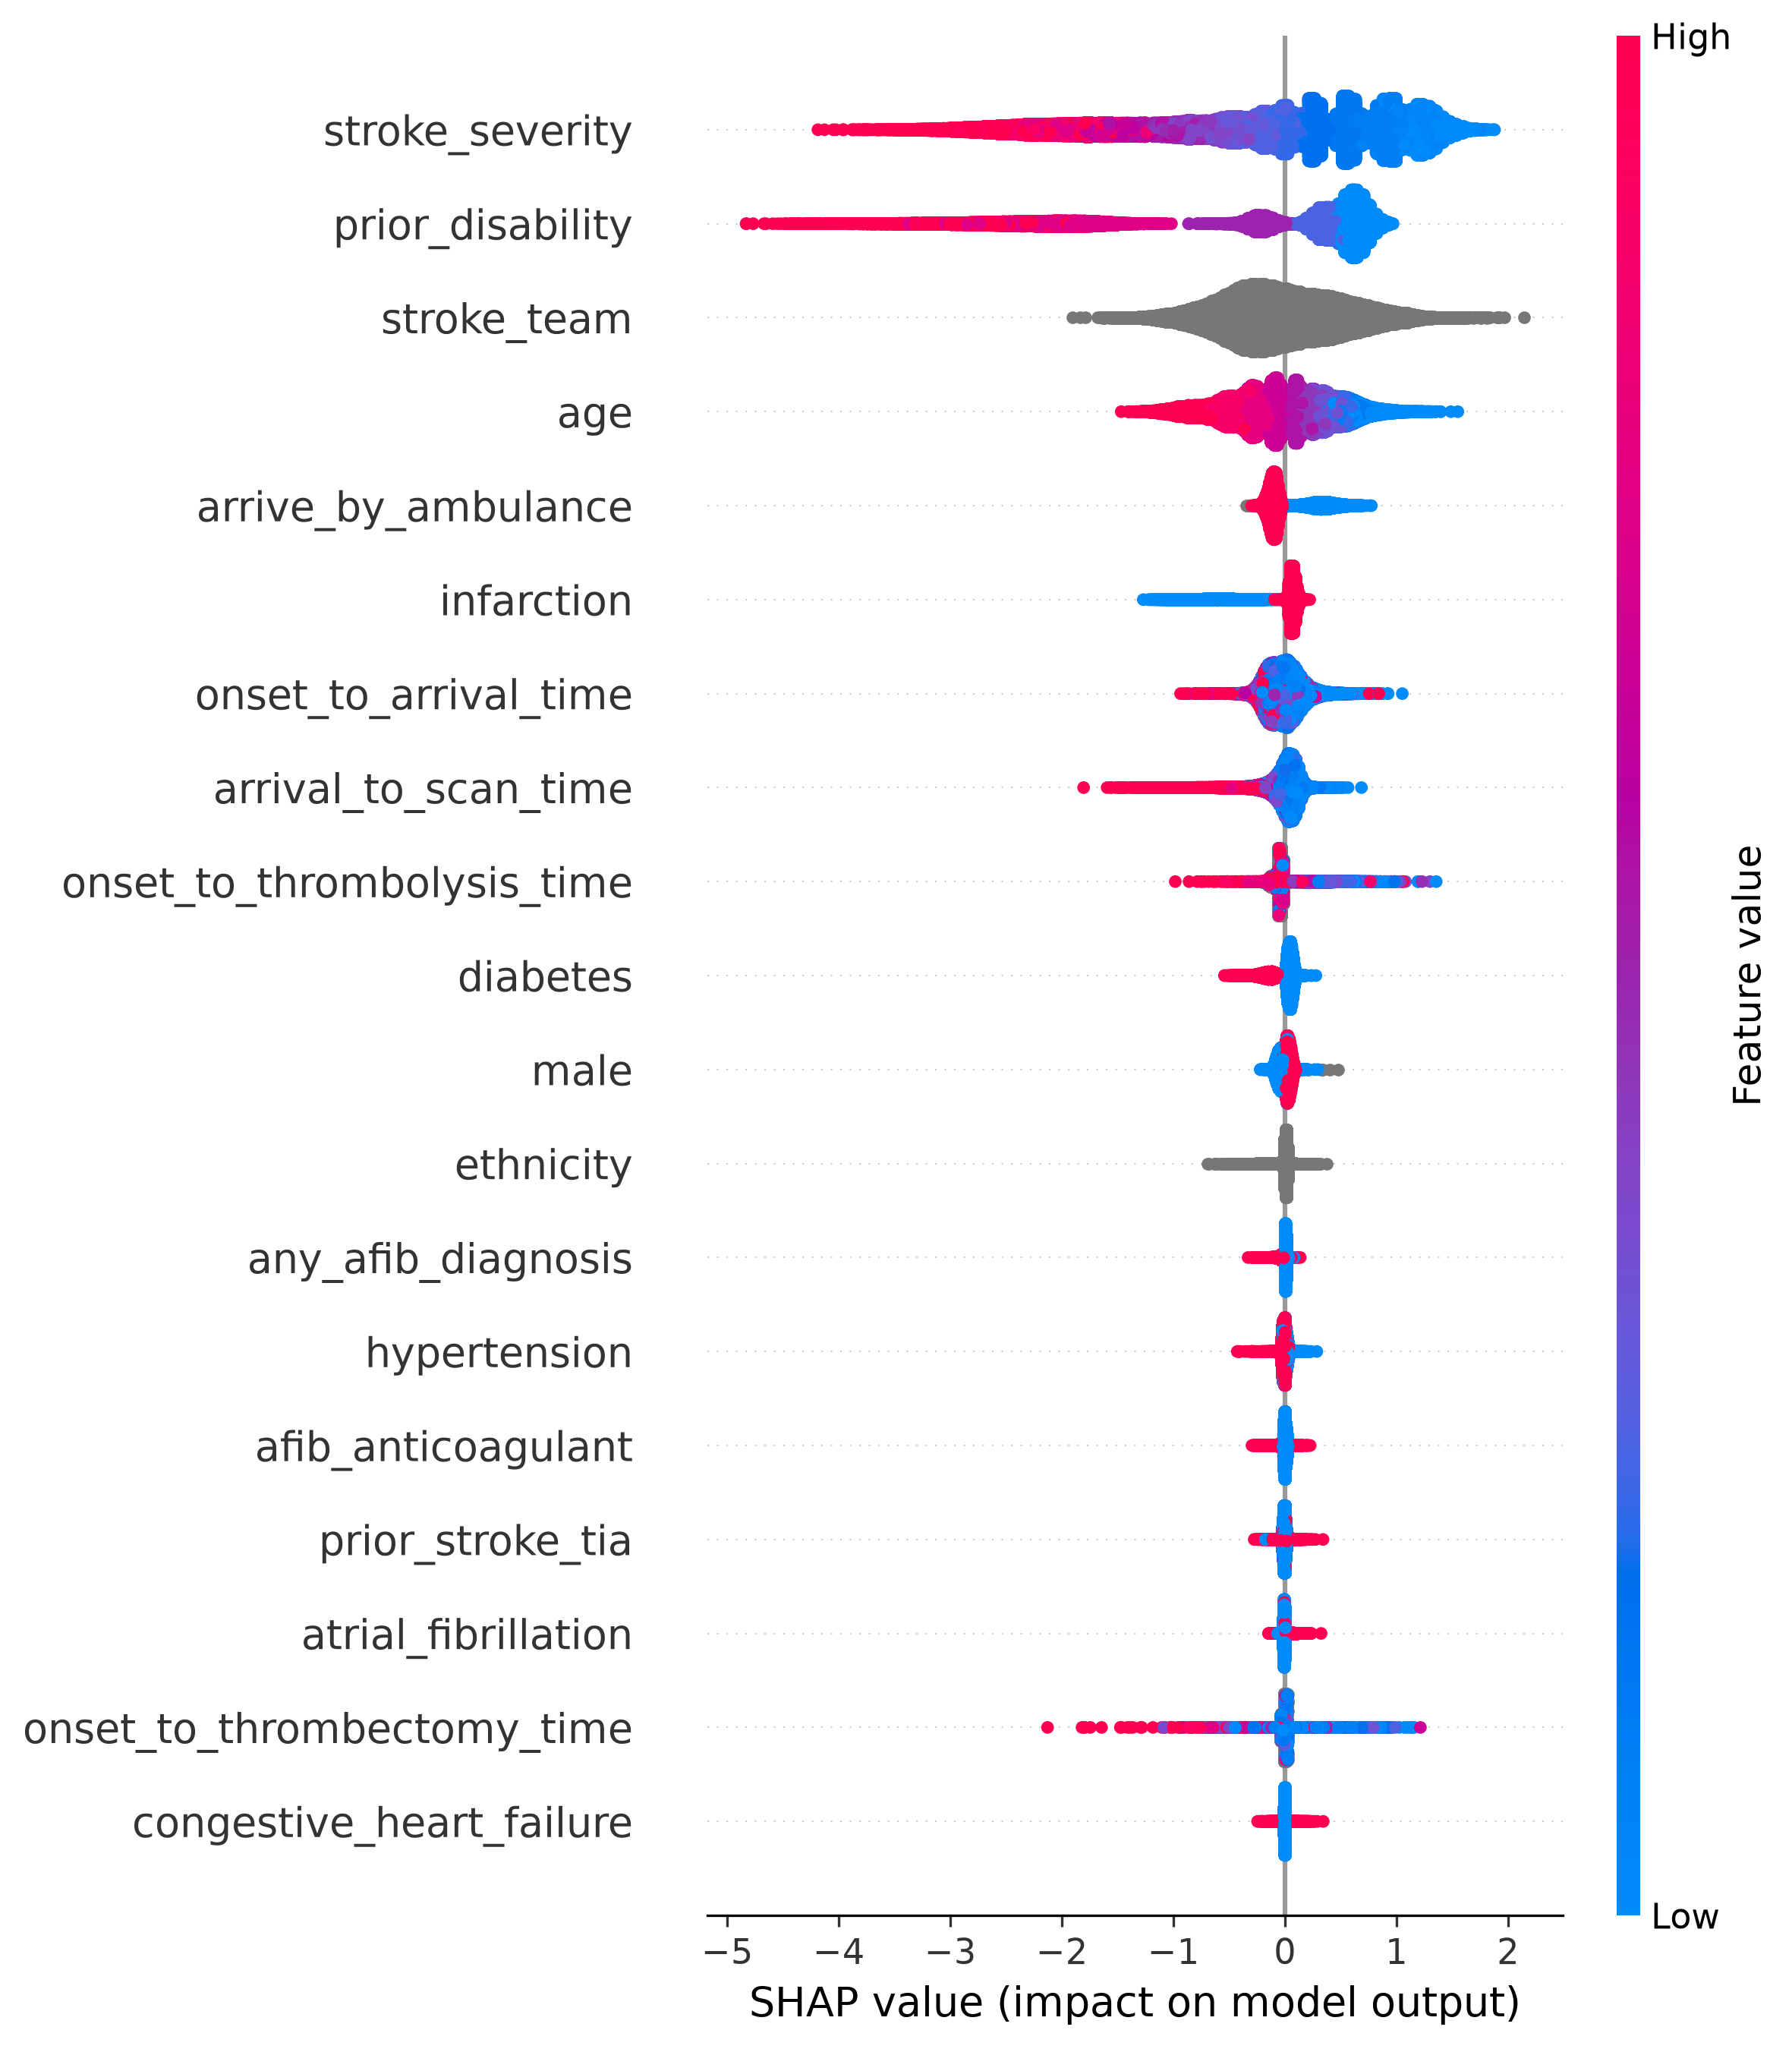
\includegraphics[width=\linewidth]{images/shap/shap_all_patients_mrs_less_than_3.png}
        %\caption{}
        \label{fig:top}
    \end{subfigure}

    \vspace{0.5cm} % Optional vertical space between rows

    % Bottom left image (~45% width)
    \begin{subfigure}{0.407\textwidth}
        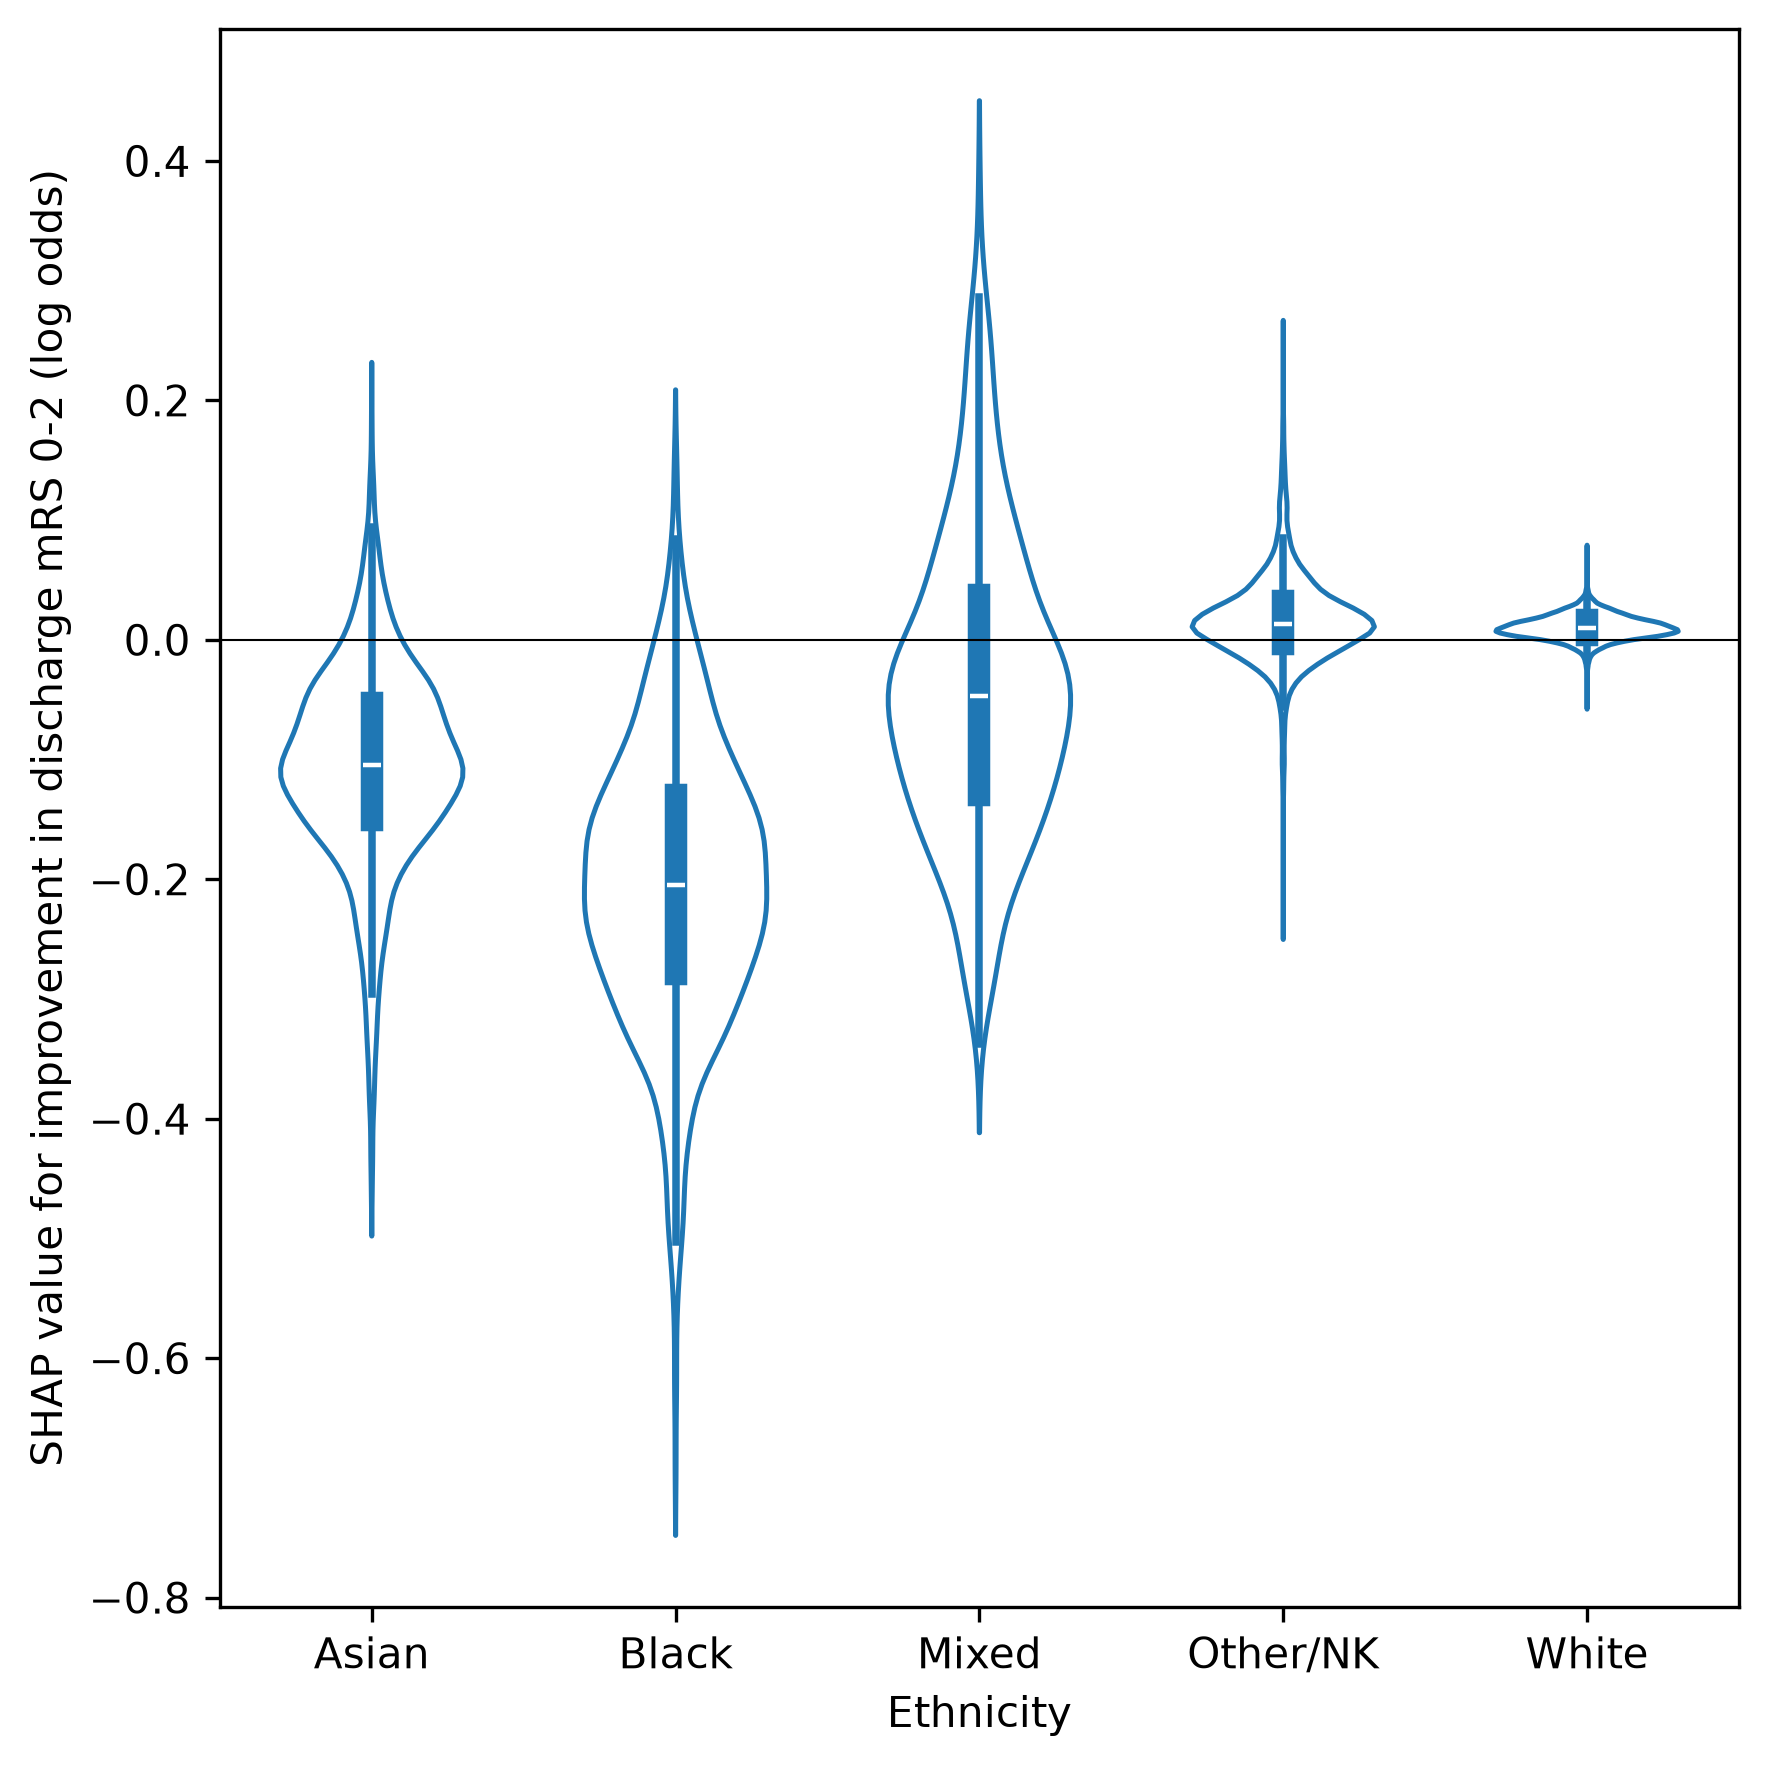
\includegraphics[width=\linewidth]{images/shap/shap_all_patients_mrs_less_than_3_ethnicity.png}
        %\caption{}
        \label{fig:bottom-left}
    \end{subfigure}
    \hfill % Adds flexible horizontal spacing
    % Bottom right image (~55% width)
    \begin{subfigure}{0.543\textwidth}
        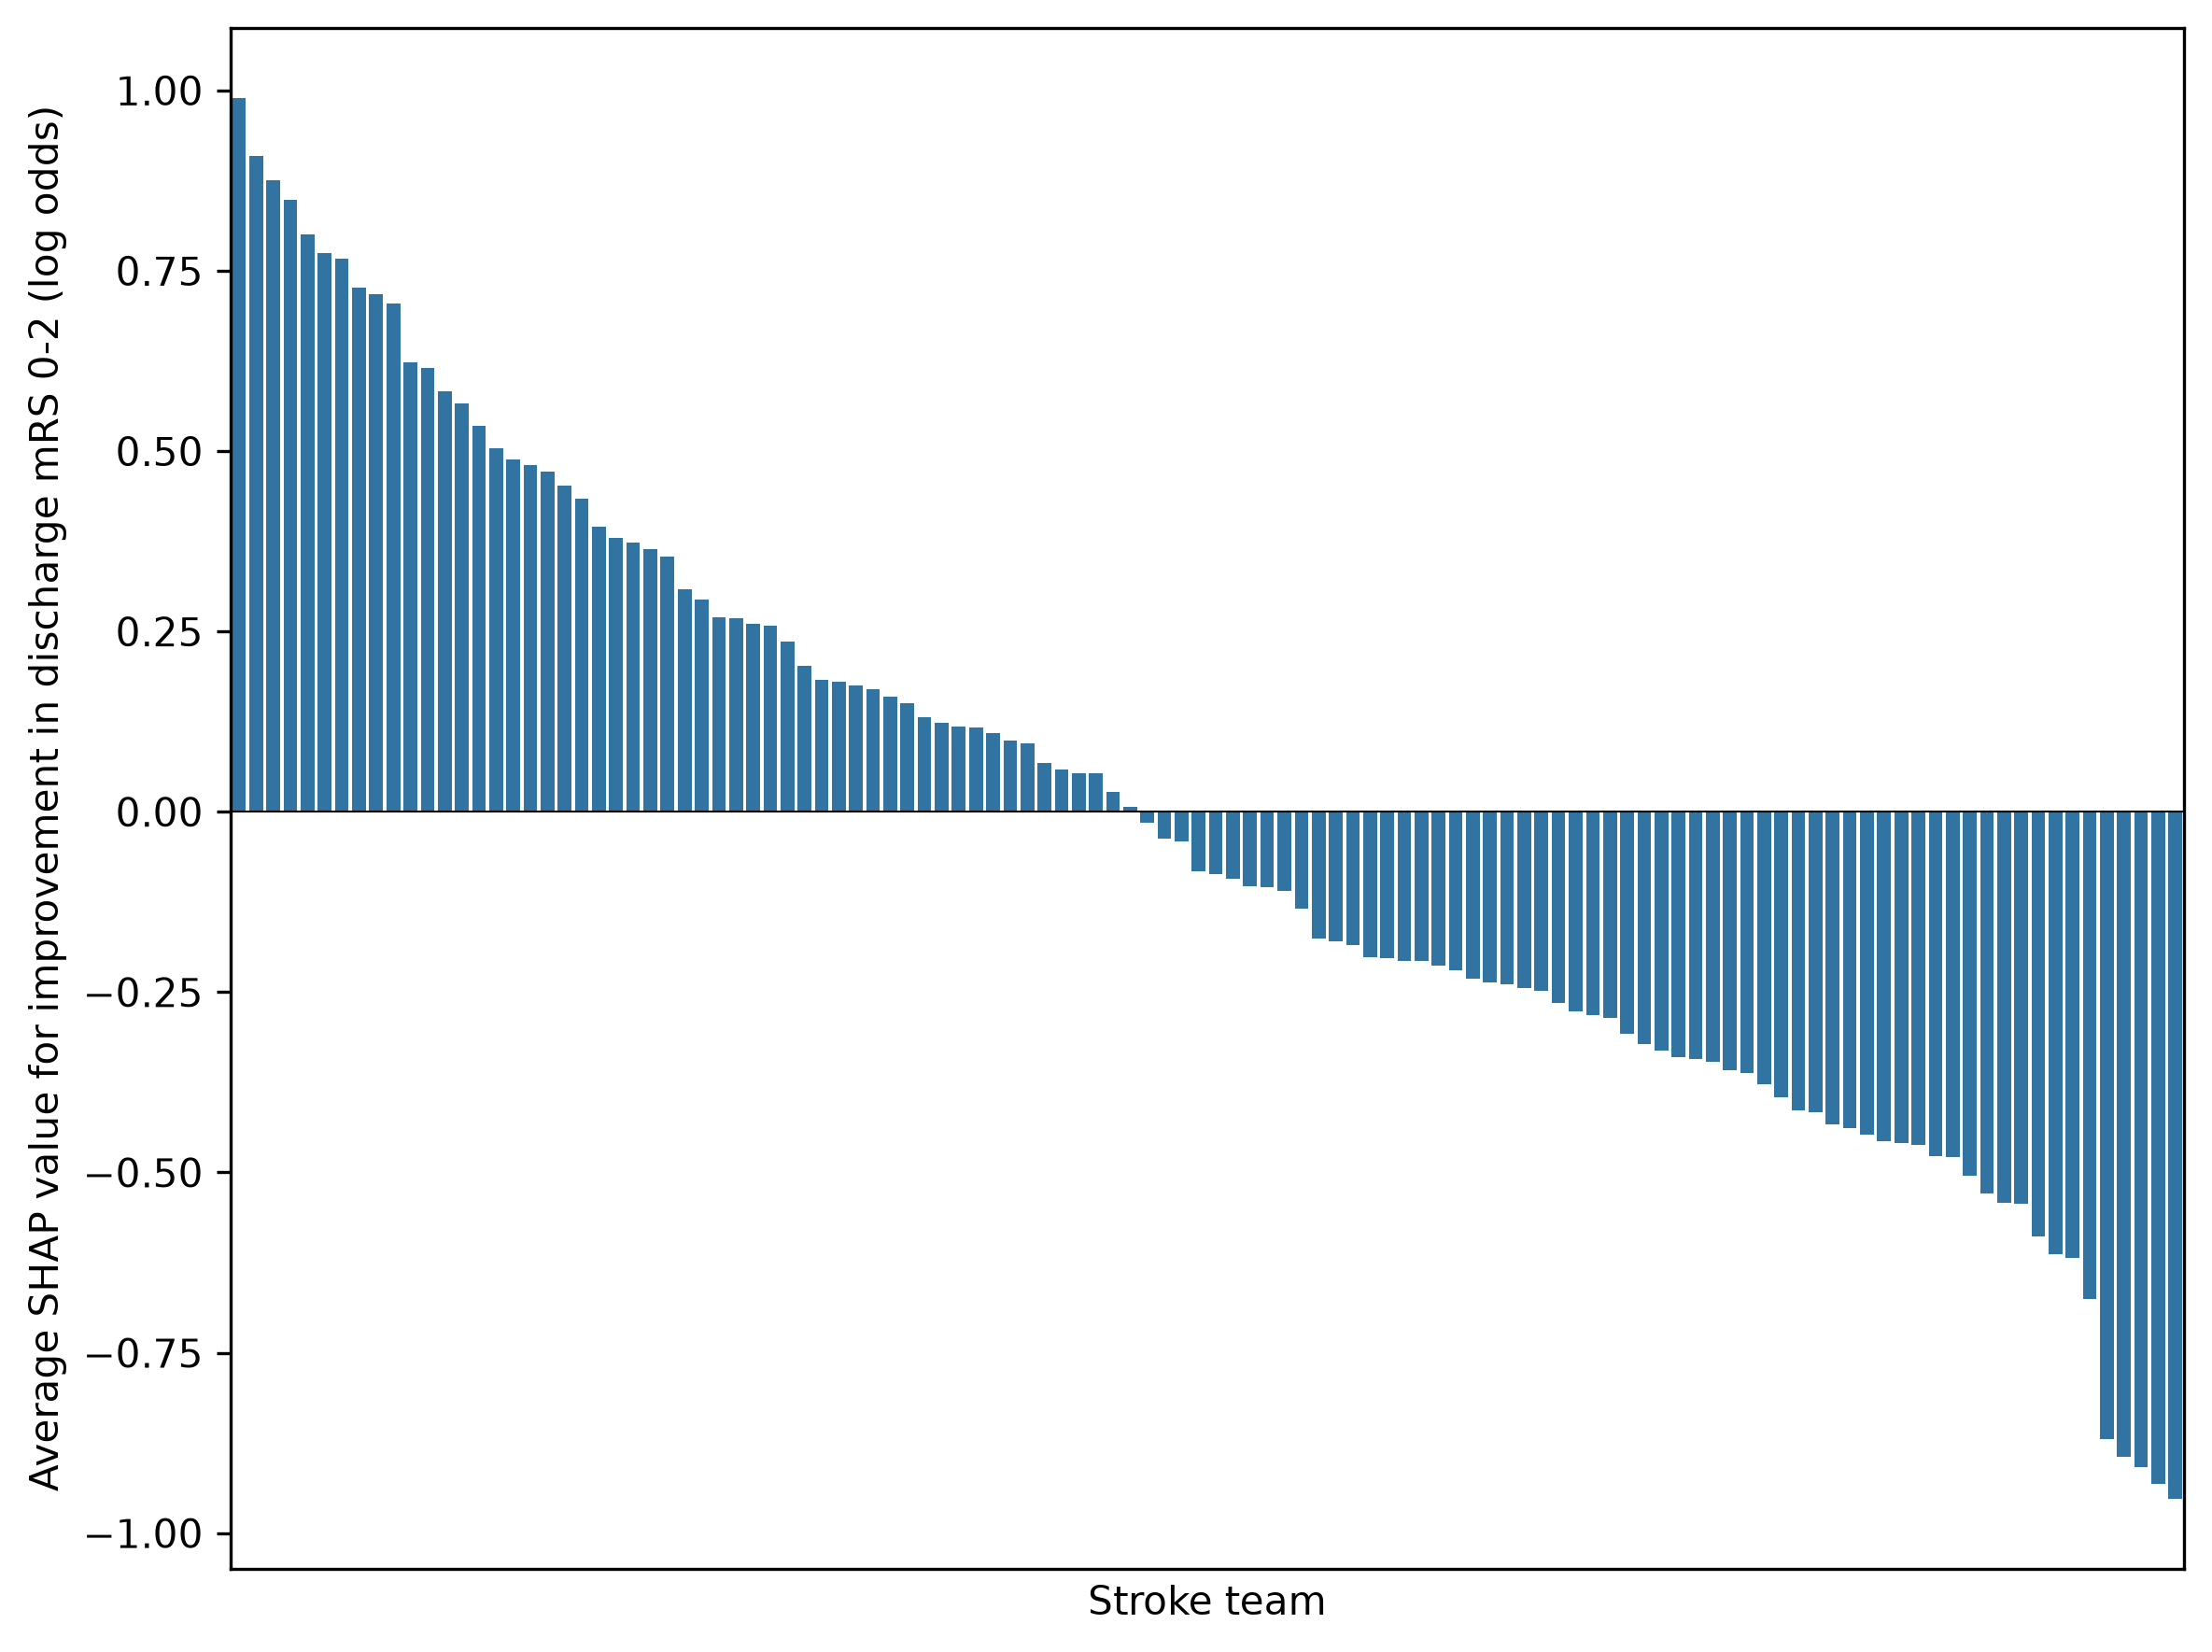
\includegraphics[width=\linewidth]{images/shap/shap_all_patients_mrs_less_than_3_stroke_team.png}
        %\caption{}
        \label{fig:bottom-right}
    \end{subfigure}

    \caption{SHAP analysis of feature contributions to predicting favourable discharge outcomes (mRS 0-2) in stroke patients. \textit{Top}: A SHAP summary plot detailing the impact of features on the model's log-odds predictions. Each point represents an individual patient instance. The position on the x-axis indicates the SHAP value, where positive values increase the predicted odds of a favourable outcome, and negative values decrease it. For continuous and binary variables, colour represents the original feature value (red indicating high values; blue indicating low values). Categorical variables (\textit{stroke team} and \textit{ethnicity}) are plotted in grey. \textit{Bottom left}: Violin plots illustrating the distribution of SHAP values across distinct ethnic groups. This panel highlights the marginal impact and variance of ethnicity on the model’s prediction for disability outcome. \textit{Bottom Right}: A ranked bar chart displaying the average SHAP value associated with each individual stroke team. This panel visualizes institutional variation, reflecting the contribution of the treating stroke team to the predicted patient outcome after accounting for patient-level clinical characteristics.}
    \label{fig:shap_all}
\end{figure}


\begin{figure}
    \centering
    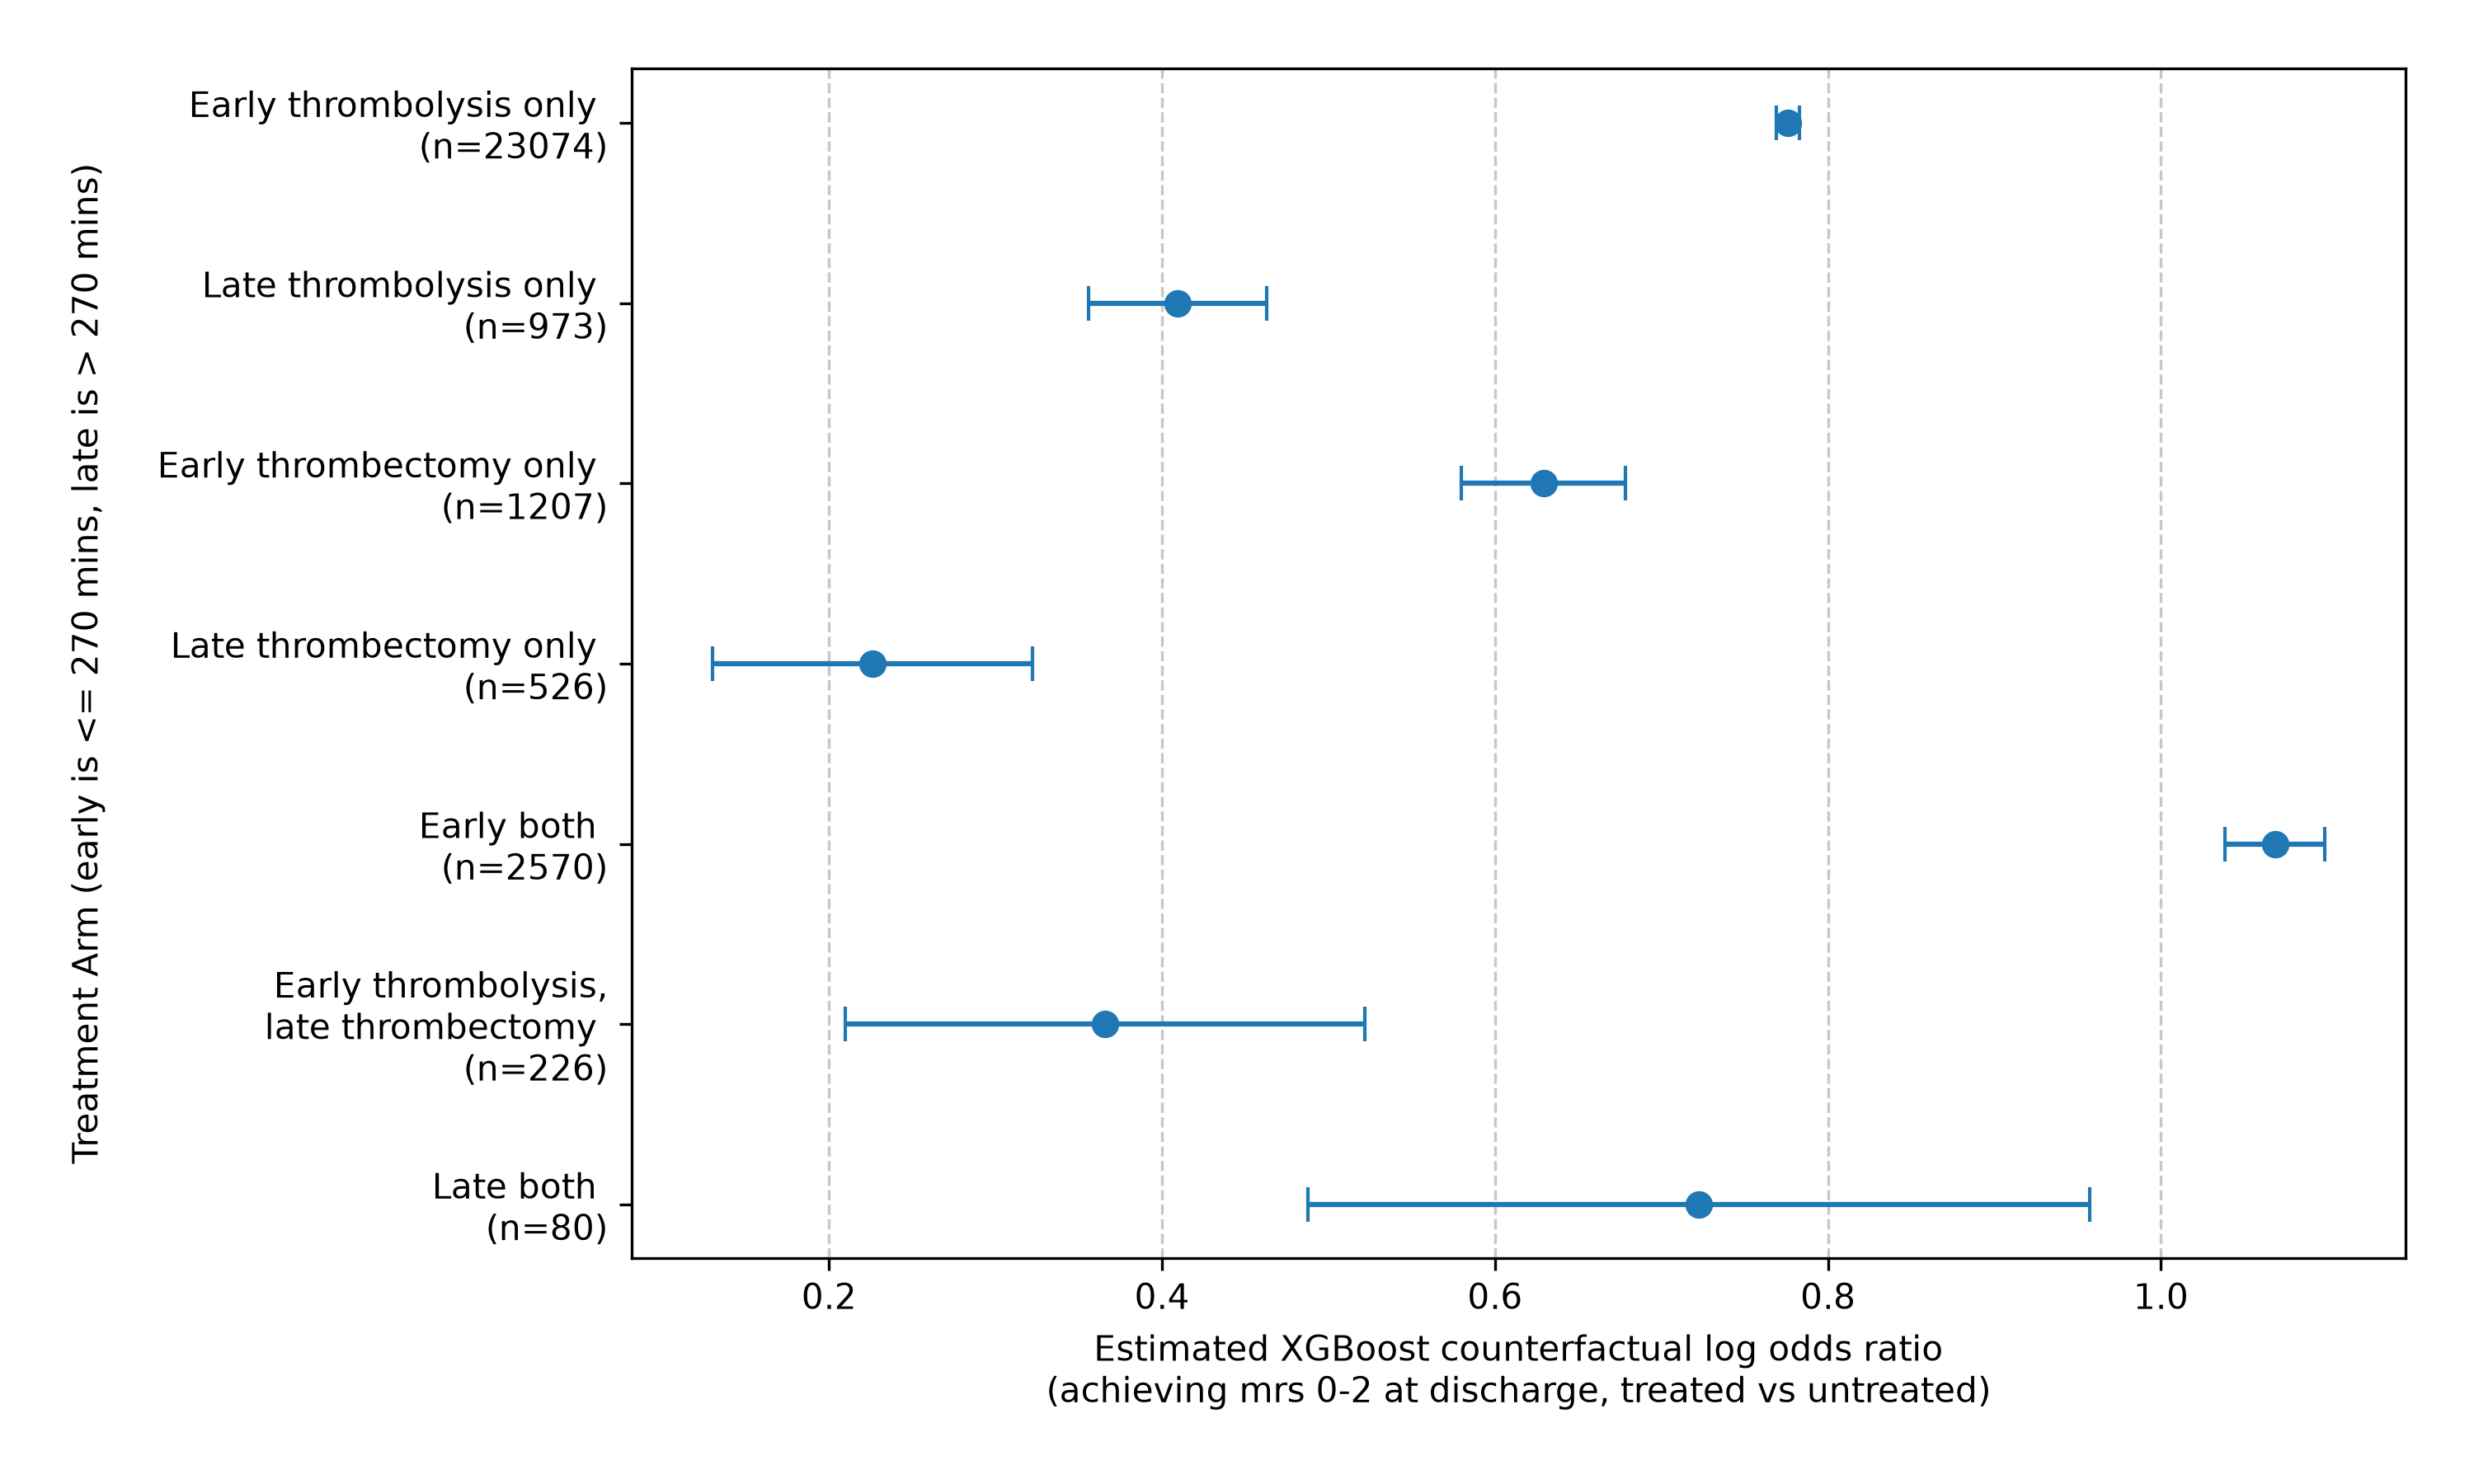
\includegraphics[width=1\linewidth]{images/treatment_effects/xgboost_counterfactual_cate_log_odds_estimates_2.png}
    \caption{Estimated counterfactual treatment benefit across reperfusion-treatment timing strategies, derived from the XGBoost S-learner model, comparing the odds of being discharged mRS 0-2 with and without treatment. Points represent the mean estimated individual treatment effect for each treatment-timing group, expressed as the counterfactual log odds ratio for being discharged mRS 0-2 relative to no reperfusion treatment; horizontal error bars show 95\% confidence intervals. Treatment groups are defined by receipt of intravenous thrombolysis and/or mechanical thrombectomy, with early treatment defined as onset-to-treatment time $<$270 minutes and late treatment as $\geq$270 minutes. Sample sizes are shown alongside group labels. Values above zero indicate a model-predicted increase in the odds of being discharged mRS 0-2 under the observed treatment strategy compared with no treatment.}
    \label{fig:main_s_learner_benefit}
\end{figure}

\subsection{Causal Forest}

\begin{figure}
    \centering
    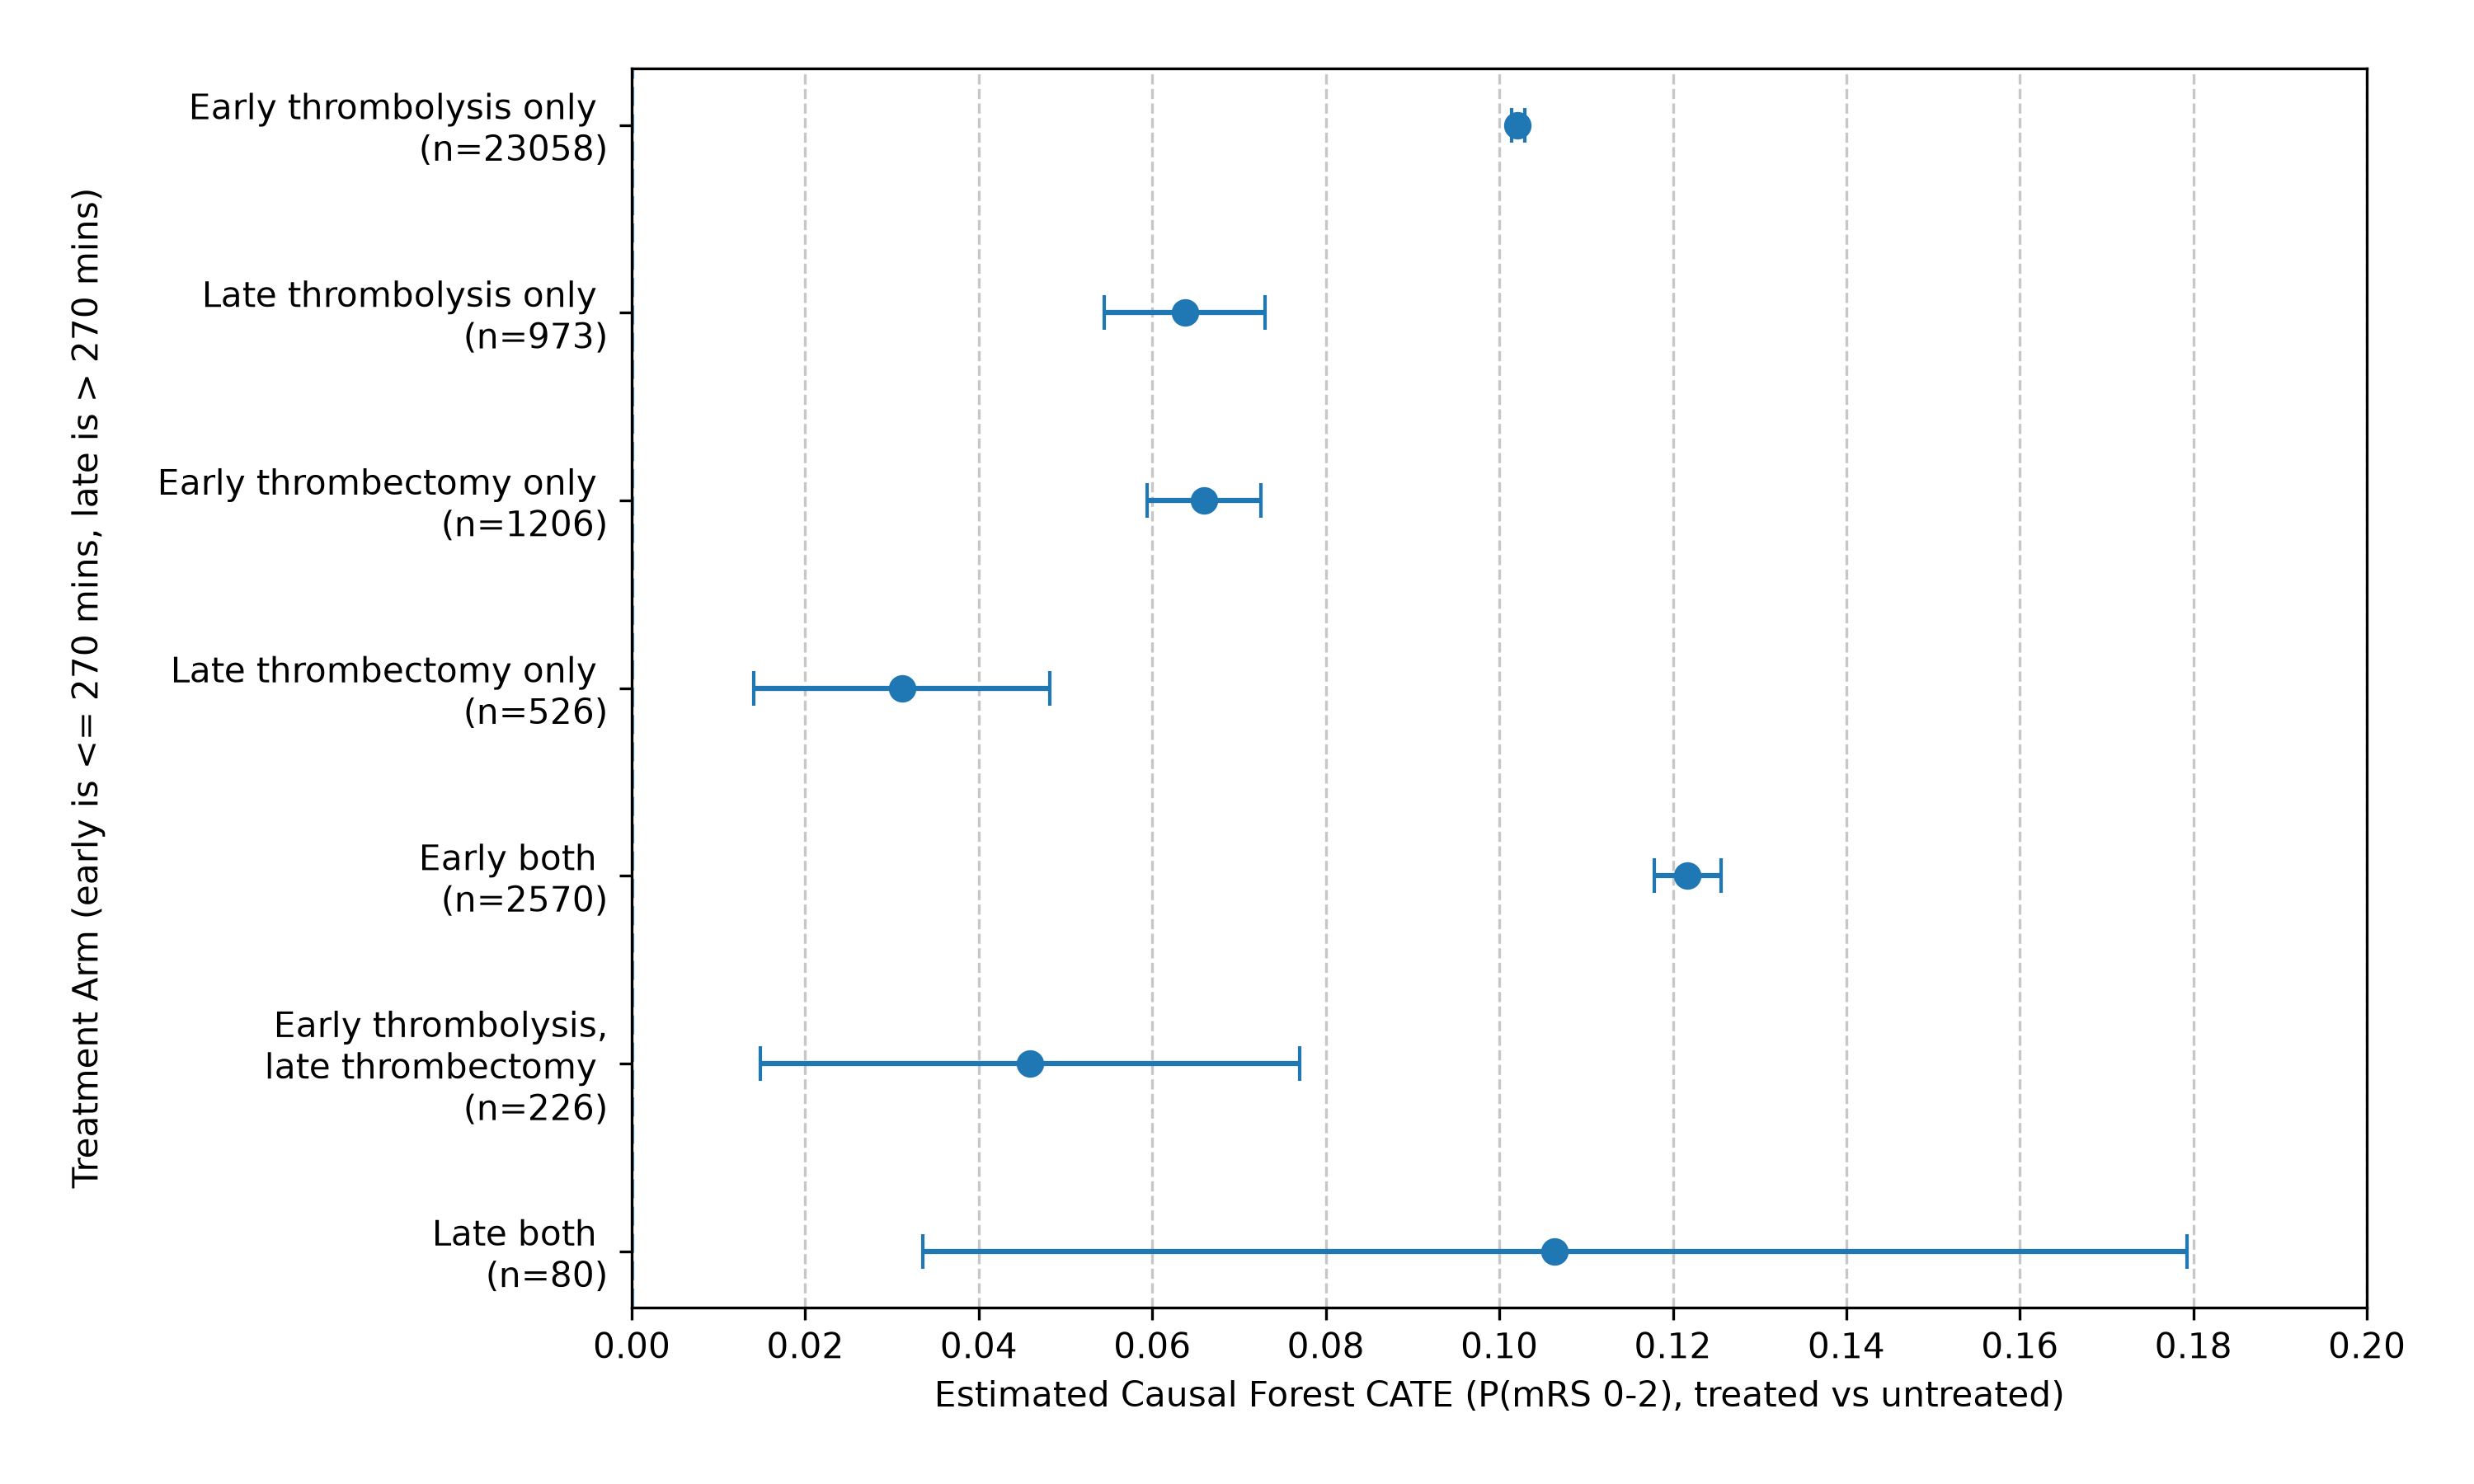
\includegraphics[width=1\linewidth]{images/treatment_effects/causal_forest_counterfactual_cate_estimates_2.png}
    \caption{Estimated counterfactual treatment benefit across reperfusion-treatment timing strategies, derived from the Causal Forest model, comparing the probability of being discharged mRS 0-2 with and without treatment. Points represent the mean estimated individual treatment effect for each treatment-timing group, expressed as the counterfactual probability improvement for being discharged mRS 0-2 relative to no reperfusion treatment; horizontal error bars show 95\% confidence intervals. Treatment groups are defined by receipt of intravenous thrombolysis and/or mechanical thrombectomy, with early treatment defined as onset-to-treatment time $<$270 minutes and late treatment as $\geq$270 minutes. Sample sizes are shown alongside group labels. Values above zero indicate a model-predicted increase in the probability of achieving the corresponding mRS outcome under the observed treatment strategy compared with no treatment.}
    \label{fig:main_causal_forest_mrs_2}
\end{figure}

